%%%%%%%%%%%%%%%%%%%%%%%%%%%%%%%%%%%%%%%
% Deedy CV/Resume
% XeLaTeX Template
% Version 1.0 (5/5/2014)
%
% This template has been downloaded from:
% http://www.LaTeXTemplates.com
%
% Original author:
% Debarghya Das (http://www.debarghyadas.com)
% With extensive modifications by:
% Vel (vel@latextemplates.com)
%
% License:
% CC BY-NC-SA 3.0 (http://creativecommons.org/licenses/by-nc-sa/3.0/)
%
% Important notes:
% This template needs to be compiled with XeLaTeX.
%
%%%%%%%%%%%%%%%%%%%%%%%%%%%%%%%%%%%%%%

\documentclass[letterpaper]{deedy-resume} % Use US Letter paper, change to a4paper for A4
\begin{document}

%----------------------------------------------------------------------------------------
%    TITLE SECTION
%----------------------------------------------------------------------------------------

% \lastupdated % Print the Last Updated text at the top right

\namesection{Zachary}{Jones}{ % Your name

% Your website, LinkedIn profile or other web address
\href{mailto:zak@newalexandria.org}{zak@newalexandria.org}  || \href{tel:+1.412.628.0954}{412.628.0954} mobile  ||  220 E. 63rd Street, New York, NY 10065
}

%----------------------------------------------------------------------------------------
%    LEFT COLUMN
%----------------------------------------------------------------------------------------

\begin{minipage}[t]{0.33\textwidth} % The left column takes up 33% of the text width of the page

%------------------------------------------------
% Education
%------------------------------------------------

\section{Education}

%------------------------------------------------

\subsection{Carnegie Mellon}

\descript{BFA; Electronic and Hypermedia}
\descript{HCI (Interface Design, Usability)}
\location{Pittsburgh, PA. May 2000}
VR/AR work, engineering arts.

\sectionspace % Some whitespace after the section

%------------------------------------------------

\subsection{Arizona State University}
\descript{MFA; HCI (Digital Technology)}
\location{Tempe, AZ. May 2007}
AR, HCI, Simulation, 3D/CNC, water.

\sectionspace % Some whitespace after the section

%------------------------------------------------
% Links
%------------------------------------------------

\section{Links}

Github:// \href{https://github.com/NewAlexandria}{\bf newalexandria} \\
LinkedIn:// \href{https://linkedin.com/in/newalexandria}{\bf newalexandria} \\
StackOverflow:// \href{https://stackoverflow.com/story/newalexandria}{\bf newalexandria} \\
Twitter:// \href{https://twitter.com/invis_insight}{\bf @invis\_insight} \\
StackNetwork:// \href{https://stackexchange.com/users/97237/new-alexandria?tab=accounts}{\bf newalexandria}

\sectionspace % Some whitespace after the section

%------------------------------------------------------------------------------

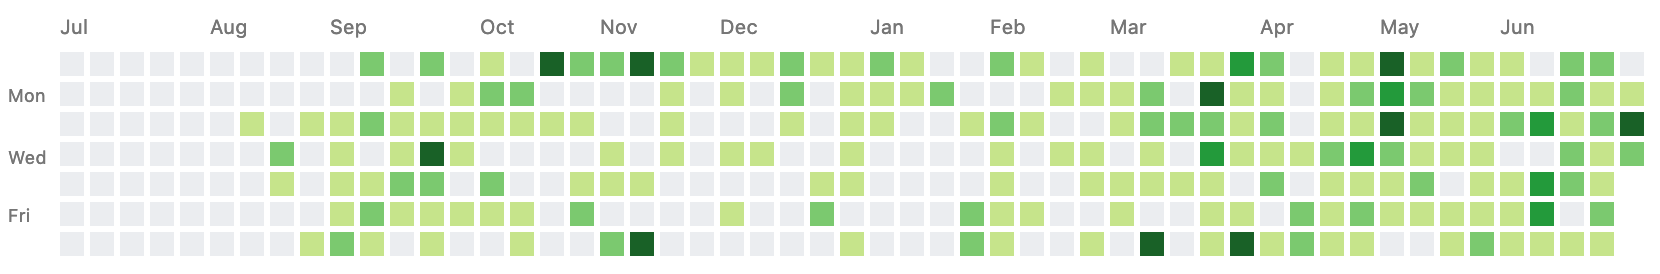
\includegraphics[width=2.3in]{github-work}

\section{}
\sectionspace % Some whitespace after the section

\section{}
\sectionspace % Some whitespace after the section

\section{}
\sectionspace % Some whitespace after the section

\section{}
\sectionspace % Some whitespace after the section

\section{}
\sectionspace % Some whitespace after the section

\section{}
\sectionspace % Some whitespace after the section

\section{}
\sectionspace % Some whitespace after the section

\section{}
\sectionspace % Some whitespace after the section

\section{}
\sectionspace % Some whitespace after the section

%------------------------------------------------
% Patent Work
%------------------------------------------------

\section{Patent Work}

\begin{tabular}{rll}
2014 & Business App Cloud\\
2010 & Crystallization Reactor\\
2008 & Vortex water\\
2007 & HRS Semantic vectors\\
\end{tabular}


\end{minipage} % The end of the left column
\hfill
%
%----------------------------------------------------------------------------------------
%    RIGHT COLUMN
%----------------------------------------------------------------------------------------
%
\begin{minipage}[t]{0.66\textwidth} % The right column takes up 66% of the text width of the page

%------------------------------------------------
% Experience
%------------------------------------------------

\section{Experience}

%------------------------------------------------

\runsubsection{<conversational templating app>}
\descript{| Lead}

\location{Mar 2017 - Feb 2018 | New York, NY}
\vspace{\topsep} % Hacky fix for awkward extra vertical space
\begin{tightitemize}
\item Research into semantic features of job-seeker emails \& time-series.
\item Hypermedia API spec in siren format, via swagger. PWA webapp in React
\item Clickable prototype. Medium-fidelity screens based on data model. UX flow.
\item Dual-appstore deploy to iOS and Android, via React Native.
\item Develop evented system. Incremental data and extraction jobs with amqp.
\end{tightitemize}

\sectionspace % Some whitespace after the section

%------------------------------------------------

\runsubsection{Investopedia}
\descript{| Director of Engineering}
\location{Dec 2017 - Aug 2018 | New York, NY}

\vspace{\topsep} % Hacky fix for awkward extra vertical space
Conversational content UI with dynamic grid UX.
\begin{tightitemize}
\item Frontend widget atomic components are stateless-cachable on vert.x + React.
\item microservice middleware in vert.x (java), Kotlin of personalization. The
\item Semantic content admin CMS with wagtail / python.
\item Spec’d CMS with stockholder. Built team; focused biz unit with GM.
\item Developed new product strategy with exec team.
\end{tightitemize}

\sectionspace % Some whitespace after the section

%------------------------------------------------

\runsubsection{MyBankTracker}
\descript{| Director of Engineering (CTO)}
\location{Oct 2015 - Dec 2017 | Brooklyn, NY}

\vspace{\topsep} % Hacky fix for awkward extra vertical space
Semantic UI on top of Personalization Engine for Financial Products
\begin{tightitemize}
\item Semantic extraction using custom model tree (CoreNLP proved too heavy).
\item NB classifier for extraction outliers. Tag for reinforcement, or auto-publishing
\item NB classifier to categorize product description sentences into semantic groups for personalized / focused UI displays.
\item Elasticsearch linked-data results (HAML) and grouped search results. (neo4j)
\item Data cleaning and processing of product ETL pipelines.
\item ML admin panels integrated seamlessly into an editorial admin (CMS).
\item Segmentation by cluster analysis (SQL, offline).  Stan test of stream modeling.
\item Data ontology formed via semiotics of consumer financial banking.

\end{tightitemize}

\sectionspace % Some whitespace after the section

%------------------------------------------------

\runsubsection{Medidata Solutions}
\descript{| Manager, Frontend Engineering}
\location{Aug 2014 - Oct 2015 | New York, NY}

Frontend and middle applications for Clinical Trials design and analysis
\vspace{\topsep} % Hacky fix for awkward extra vertical space
\begin{tightitemize}
\item Angular js and MVC Architecture.
\item Made a highly configurable grid rendering system for Angular
\item Set process standards, 150-200\% productivity gains.

\item Devised new behavioral analytic measures, driving product design.
\item Cucumber BDD best practices, from 3-amigos feature to agile standards.
\item Designed and executed an 8-layer QA automatiomn. Niche tools and strategies.
\item NYC Office lead for Programming Foundations Guild, Frontend Guild. 
\item Hosted conferences, external speakers, etc.

\end{tightitemize}

\sectionspace % Some whitespace after the section


%------------------------------------------------

\runsubsection{PageUI}
\descript{| Co-Founder, CTO}
\location{Jun 2008 - Mar 2009 | Tempe, AZ}

\vspace{\topsep} % Hacky fix for awkward extra vertical space
Drag'n'drop UI/UX for bookmark management and workflow
\begin{tightitemize}
\item Developed early reactive-JS codebase, and stacked our app/biz on it.
\item Mozilla later supported a nearly identical labs project, with major adoption.
\item Usabilty research showed preference over X-marks, which was mainstream.
\end{tightitemize}

\sectionspace % Some whitespace after the section
%----------------------------------------------------------------------------------------

\end{minipage} % The end of the right column

%----------------------------------------------------------------------------------------
%    SECOND PAGE (EXAMPLE)
%----------------------------------------------------------------------------------------

\newpage % Start a new page

\begin{minipage}[t]{0.33\textwidth} % The left column takes up 33% of the text width of the page

%------------------------------------------------
% Awards
%------------------------------------------------

\section{Awards}

\begin{tabular}{rll}
2019 & \textbf{M\&A exit:} Personalization\\
2008 & NASA/Ames Arts \& Engineering\\
2007 & Grant for CFD analysis\\
2006 & Seed capital raised: Edson\\
2006 & Art \& Engineer Talent Award\\
2005 & Various lecture travel grants\\
2003 & Contrib: Ag. grants for \$2MM\\
1999 & Building Virtual Worlds grant\\
1998 & Sonoluminescence lab grant\\
\end{tabular}

\sectionspace % Some whitespace after the section

%------------------------------------------------
% Societies
%------------------------------------------------

\section{Societies}

\begin{tabular}{rll}
2015-2019 & Papers We Love\\
2004-2019 & PEAR Lab \& ICRL\\
2006 & SkySong Accelerator\\
2005-2007 & AME assn. President\\
1996-1999 & CMU Student Senator\\
1998-1999 & Stage 3 Lab\\
\end{tabular}

\sectionspace % Some whitespace after the section

%------------------------------------------------
% Publications
%------------------------------------------------

\section{Publications}

\begin{tabular}{rll}
2018 & RPA Summit\\
2017 & AI World\\
2009 & Filters \& Reflections anthology\\
2007 & AZ State STEM curriculum WG\\
2007 & Technoetic Arts Journal\\
2004 & Qi and Complexity, Beijing\\
2001 & Phytoremediation, Dept. Energy\\
\end{tabular}

\sectionspace % Some whitespace after the section

\end{minipage} % The end of the left column
\hfill
\begin{minipage}[t]{0.66\textwidth} % The right column takes up 66% of the text width of the page

%------------------------------------------------
% Research
%------------------------------------------------

\section{Research \& Projects}

%------------------------------------------------

\runsubsection{Cloud App Platform}
\descript{| R\&D Engineering}
\location{Jun 2013 - Oct 2015 | New York, NY}

\vspace{\topsep} % Hacky fix for awkward extra vertical space
\begin{tightitemize}
\item Designed lambda-as-a-service pattern for data-platform strategy.
\item Won trust with executive backers, started working group.
\item Developed patent strategy with chief patent counsel.
\item Two separte R\&D initiatives across Pharma and Financial Data corps.
\end{tightitemize}

\sectionspace % Some whitespace after the section


%------------------------------------------------

\runsubsection{Bardcruft}
\descript{| Situated Media programme}
\location{2004, 2017 | Tempe; NYC}

UX Design and systems for finding similarities in narratives (‘Hero of 100 Faces’)
\begin{tightitemize}
\item Use of ConceptNet, mysql (now RDF4J and SPARQL)
\item Translation of stories into state trajectories and relationship triples
\item Visualization of semantic graph by-concept (scopes/filters)
\item Text annotation GUI for creating new triples.
\end{tightitemize}

\sectionspace % Some whitespace after the section


%------------------------------------------------


\runsubsection{Convergance study of CFD + Experimental Data}
\descript{| ASU}

\location{June 2006 - Oct 2009 | Tempe, AZ}
\vspace{\topsep} % Hacky fix for awkward extra vertical space
Multiple studies of a non-turbulent vortex hydrodynamic equilibrium.
\begin{tightitemize}
\item Algorithmic model development in python and CAD machining.
\item CFD modeling with ANSYS multiphysics.
\item Quantified comparison k-$\epsilon$ turbulence, reynolds stress, and laminar simulations.
\item Analysis of free-surface experimental model, and simulation data.
\item Platform patent strategy.  Grants. Seed capital raised. Team of world authorities.
\end{tightitemize}

\sectionspace % Some whitespace after the section

%------------------------------------------------

\runsubsection{Biophoton and QED research visualization.}
\descript{| ASU }

\location{Aug 2008 | Tempe, AZ}
\begin{tightitemize}
\item Designed codes for conversion of analytic protein data into physical model.
\item Worked with 3D data in PDB and OBJ formats from the \textit{wwPDB} database.
\item Designed and programmed of 3D computer graphic algorithms in numpy.
\item Averaging series of femtosecond datasets from HPCI/MPI simulations.
\item Solid model files for printing via FDM rapid prototyping on Stratasys hardware.
\end{tightitemize}

\sectionspace % Some whitespace after the section


%------------------------------------------------


\runsubsection{HRS}
\descript{| Co-Founder, CTO}

\location{Jan 2006 - Oct 2007 | Vancouver, BC}
\begin{tightitemize}
\item Designed search and matching algorithms for social search.
\item Semantics modeled as state vectors for protocol engineering.  Pre-blockchain.
\item Performed prior-art research and wrote a draft patent. IP law firm counsel.
\item Developed a collaboration-ware app for course software, distance education.
\end{tightitemize}

\sectionspace % Some whitespace after the section

%------------------------------------------------

\runsubsection{TensorVision}
\descript{| ASU, Sponsored Research}

\location{Sept 2005 – May 2006 | Tempe, AZ}
\begin{tightitemize}
\item Formulated UI/UX notation conventions for data navigational affordances.
\item Aimed at creating consistent semantic meaning in 2D and 3D spaces through quantizing hypermedia datasets using mereological models.
\item Research into cognitive continuum across UX haptic and perceptual domains.
\item Live test subject research, HCI methods.  Patentable, never filed.
\end{tightitemize}

\sectionspace % Some whitespace after the section


%------------------------------------------------



\end{minipage} % The end of the right column

%----------------------------------------------------------------------------------------

\end{document}
